\hypertarget{simplex_8cpp}{\section{\-Dokumentacja pliku simplex.\-cpp}
\label{simplex_8cpp}\index{simplex.\-cpp@{simplex.\-cpp}}
}


\-Definicje poszczegolnych funkcji dla klasy \hyperlink{class_simplex}{\-Simplex}.  


{\ttfamily \#include \char`\"{}simplex.\-h\char`\"{}}\*
\-Wykres zależności załączania dla simplex.\-cpp\-:
\nopagebreak
\begin{figure}[H]
\begin{center}
\leavevmode
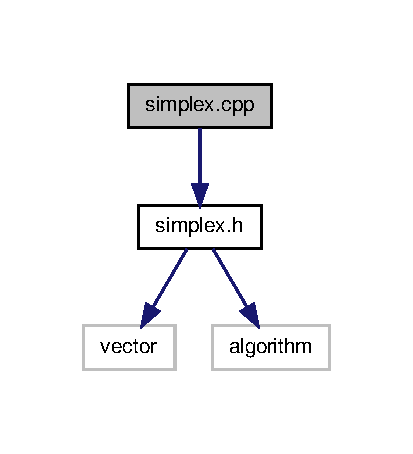
\includegraphics[width=198pt]{simplex_8cpp__incl}
\end{center}
\end{figure}


\subsection{\-Opis szczegółowy}
\-Definicje poszczegolnych funkcji dla klasy \hyperlink{class_simplex}{\-Simplex}. 

\-Definicja w pliku \hyperlink{simplex_8cpp_source}{simplex.\-cpp}.

